\documentclass[12pt,oneside]{article} % Uma Coluna e lingua portuguesa
%\usepackage[T1]{fontenc}        % Permite digitar os acentos de forma normal
\usepackage[utf8]{inputenc}
%\usepackage[english]{babel}
% \usepackage[portuges,brazil]{babel}
\usepackage[brazilian]{babel}

%\usepackage[latin1]{inputenc}
\usepackage[dvips]{graphicx}    % Permite Gráficos
%\usepackage{times}    % Fonte Times
\usepackage{fancyhdr}
\usepackage{array}
\usepackage{multicol}
\usepackage[colorlinks=true,linkcolor=blue,urlcolor=blue]{hyperref}
\usepackage{nomencl}    % glossario
\usepackage{amssymb}
\usepackage{amsmath}
\usepackage[compact]{titlesec}
\usepackage{wrapfig}
\usepackage{color}
\usepackage{csquotes}

%=======================================================================

% Hifenização das palavras desconhecidas pelo LaTeX
%\hyphenation{}
\paperheight    297mm
\paperwidth     210mm
\voffset         -15mm
\headheight      15pt %% tamanho de letra
\headsep         5mm  %% para o início do texto
\oddsidemargin  -3.0mm
\evensidemargin -3.0mm
\textwidth      167.0mm
\topmargin      005.0mm
\textheight     240.0mm
\footskip       10.0mm

\title{SAET 2024 - Maratona de Programação}

\author{Maratona de Programação}
\date{29 de novembro de 2024}
\usepackage{indentfirst}
\usepackage{subfig}

\parindent=0pt
\setlength{\parskip}{7pt plus 1pt minus 2pt}
\titlespacing{\section}{0pt}{*0}{*0}
\titlespacing{\subsection}{0pt}{*0}{*0}
\titlespacing{\subsubsection}{0pt}{*0}{*0}

\begin{document}

\begin{center}
\textbf{\Huge SAET 2024 - Maratona de Programação} \\
\vspace{0.2cm}
\textit{29 de novembro de 2024} \\
\vspace{1.0cm}
%\textbf{Sevidor BOCA:} \\
%\texttt{\large http://maratona.c3sl.ufpr.br/boca/} \\
%\vspace{1.0cm}
\begin{figure}[h!]
	\centering
 
\includegraphics[scale=0.95]{capa.png}
\end{figure}
\vspace{1.0cm}
%\textbf{Organizadores:}\\
%{\small Flávio Zavan} \\
%{\small Ricardo Oliveira} \\
\vspace{1.0cm}
\end{center}

\clearpage

\pagestyle{fancy}
\renewcommand{\footrulewidth}{0.7pt}
\renewcommand{\headrulewidth}{0.7pt}
\lhead{SAET 2024}
\chead{Maratonas de Programação}
\rhead{29 de novembro de 2024}
\cfoot{\thepage}

\newpage

% Espaco para o create-zips.sh nao achar
  \section*{Instruções Importantes}

\begin{itemize}

    \item Use a opção \textbf{Runs} para enviar suas soluções. Os problemas podem resolvidos em qualquer ordem e
    linguagem (dentre C, C++ e Python, independentemente do problema);

    \item Suas soluções serão testadas com várias entradas,
    além das dada como exemplo. Por isso, sua solução pode não ser
    aceita mesmo se funcionar para os exemplos dados. Certifique-se que ela
    funciona para todas as entradas possíveis;

    \item A saída gerada deve ser \textit{exatamente} conforme
    especificada. Em particular, \textbf{não} imprima instruções (``digite um
            número'', ``a resposta é'', etc);

    \item É garantido que todas as entradas usadas para teste estarão de acordo
    com o enunciado, não sendo necessário testar se são válidas;

    \item Ao enviar uma solução, o sistema irá responder uma das
    seguintes respostas:
    \begin{itemize}
        \item \verb|Not answered yet|: a solução está sendo corrigida.
        Aguarde um pouco e atualize a página;
        \item \verb|YES|: solução aceita. Parabéns!
        \item \verb|Wrong Answer|: a saída impressa pelo seu programa não é a
        saída correta esperada, para alguma entrada de teste;
        \item \verb|Presentation Error|: a saída impressa está correta, exceto
        por espaços em branco e/ou quebras-de-linha faltando/sobrando;
        \item \verb|Time Limit Exceeded|: o tempo de execução do seu programa
        ultrapassou o tempo limite estipulado para o problema (ver tabela
        abaixo). O tempo de execução da sua solução precisa ser menor;
        \item \verb|Runtime Error|: seu programa gerou algum erro em tempo de
        execução (``crashou'');
        \item \verb|Compile Error|: seu programa não compila.
    \end{itemize}

    \item Todas as linhas, tanto na entrada quanto na saída, terminam com o
    caractere de fim-de-linha ($\backslash n$), mesmo quando houver apenas uma única
    linha na entrada e/ou saída;

    \newpage
    \item Sua solução deve processar cada arquivo de entrada no tempo máximo
    estipulado para cada problema, dado pela seguinte tabela:

    \begin{table}[h]
    \centering
    \begin{tabular}{|c|c||c|}
    \hline
    \textbf{Problema} & \textbf{Nome} & \textbf{Tempo Limite (segundos)} \\
    \hline
    A & A Dupla do Crime & 1 \\
    B & Bisbilhoteira & 1 \\
    C &  & 1 \\
    D &  & 1 \\
    E &  & 1 \\
    F & Fibonacci & 1 \\
    G & Geoguessr & 1 \\
    H &  & 1 \\
    I &  & 1 \\
    J & Jogo da Forca & 1 \\
    K & Kummirub & 1 \\
    L &  & 1 \\
    \hline
    \end{tabular}
    \end{table}

\end{itemize}

\newpage
\section*{A: A Dupla do Crime} %tle=1
\vspace{-0.52cm}
\noindent \begin{verbatim}Arquivo: a_dupla_do_crime.[c|cpp|py]\end{verbatim}
Kubitschek e Chekskubit são os dois cachorros vira-latas que compõem a dupla de notórios criminosos procurados pelos seus terríveis, impiedosos, horripilantes, amedrontadores e imperdoáveis crimes cometidos nos arredores da UFOP (Universidade Fictícia do Oeste do Paraná). Entre os crimes realizados pela dupla, o que mais tomou notoriedade foi o de cometer, mais de uma vez, o ato terrorista de comer restos de refeições ofertados pelos alunos do campus, que, caso contrário, seriam despejados no lixo.

Diante desse crime abominável, um dos setores da UFOP, o RUF (Restaurante Universitário Fictício), entrou em contato com as autoridades e cobrou que tomassem providências contra esses bandidos perigosíssimos. Em resposta, a polícia iniciou uma campanha para capturá-los, imprimindo panfletos de "procurado" com recompensas para quem os entregasse.

Cada um dos panfletos contém as seguintes proporções:
\begin{itemize}
    \item O panfleto de Kubitschek tem proporção de altura/largura igual a 5:3.
    \item O panfleto de Chekskubit tem proporção de altura/largura igual a 3:2.
\end{itemize}

Você foi contratado para ajudar a polícia a descobrir quantos panfletos de Kubitschek e Chekskubit podem ser impressos em uma cartolina retangular de dimensões $X:Y$, de modo que a diferença entre a quantidade de panfletos de cada um dos criminosos não seja maior que 1 (ou seja, a quantidade de panfletos de Kubitschek e Chekskubit deve ser a mais equilibrada possível). Além disso, cada panfleto, seja de Kubitschek ou de Chekskubit, deve ter uma área igual a 5\% da área total da cartolina.

\subsection*{Ilustração dos panfletos}

\begin{center}
    
\includegraphics[width=0.3\textwidth]{a_dupla_do_crime/kubitschek.png}
    \hspace{1cm}
    
\includegraphics[width=0.3\textwidth]{a_dupla_do_crime/chekskubit.png}
\end{center}

\subsection*{Entrada}
A entrada consiste de dois inteiros $X$ e $Y$ representando as dimensões da cartolina $(1 \leq X, Y \leq 10^9)$.

\subsection*{Saída}
A saída deve consistir de um único número inteiro representando a quantidade máxima de panfletos de Kubitschek e Chekskubit que podem ser impressos na cartolina.


\newpage
\section*{B: Bisbilhoteira} %tle=1
\vspace{-0.52cm}
\noindent \begin{verbatim}Arquivo: bisbilhoteira.[c|cpp|py]\end{verbatim}
Nossa amiga Ana está enfrentando um problema curioso. Ela tem uma irmã bisbilhoteira que insiste em ler o seu diário sempre que tem a oportunidade. Para evitar que seus segredos sejam descobertos, Ana começou a codificar suas mensagens, repetindo os caracteres para deixar as frases mais confusas. Por exemplo, em vez de escrever ``amor", ela pode escrever ``aaammmoorrrr".

No entanto, agora ela está com outro problema: as mensagens ficaram muito grandes, ocupando páginas inteiras do diário. Para ajudar Ana, precisamos criar um algoritmo que compacte essas mensagens, substituindo as sequências de caracteres repetidos pelo caractere seguido pelo seu numero de repetições.
\subsection*{Entrada}

A entrada consiste de um numero $n$ ($1 \leq n \leq 100$) indicando o tamanho da string, seguido pela string $s$, composta apenas por letras minusculas sem espaços.

\subsection*{Saída}

Uma linha contendo a string codificada.

%----- Exemplo 1 -----%
\begin{table}[!h]
\centering
\begin{tabular}{|l|l|}
\hline
\begin{minipage}[t]{3in}
\textbf{Exemplo de entrada}
\begin{verbatim}
10 aaaaabbccc
\end{verbatim}
\vspace{1mm}
\end{minipage}
&
\begin{minipage}[t]{3in}
\textbf{Exemplo de saída}
\begin{verbatim}
a5b2c3
\end{verbatim}
\vspace{1mm}
\end{minipage} \\
\hline
\end{tabular}
\end{table}

%----- Exemplo 2 -----%
\begin{table}[!h]
\centering
\begin{tabular}{|l|l|}
\hline
\begin{minipage}[t]{3in}
\textbf{Exemplo de entrada}
\begin{verbatim}
8 ppppccii
\end{verbatim}
\vspace{1mm}
\end{minipage}
&
\begin{minipage}[t]{3in}
\textbf{Exemplo de saída}
\begin{verbatim}
p4c2i2
\end{verbatim}
\vspace{1mm}
\end{minipage} \\
\hline
\end{tabular}
\end{table}

%----- Exemplo 2 -----%
\begin{table}[!h]
\centering
\begin{tabular}{|l|l|}
\hline
\begin{minipage}[t]{3in}
\textbf{Exemplo de entrada}
\begin{verbatim}
1 a
\end{verbatim}
\vspace{1mm}
\end{minipage}
&
\begin{minipage}[t]{3in}
\textbf{Exemplo de saída}
\begin{verbatim}
1a
\end{verbatim}
\vspace{1mm}
\end{minipage} \\
\hline
\end{tabular}
\end{table}



%\newpage
%\section*{C:} %tle=1
%\vspace{-0.52cm}
%\noindent \begin{verbatim}Arquivo: .[c|cpp|py]\end{verbatim}
%\input{/.tex}


%\newpage
%\section*{D:} %tle=1
%\vspace{-0.52cm}
%\noindent \begin{verbatim}Arquivo: .[c|cpp|py]\end{verbatim}
%\input{/.tex}

%\newpage
%\section*{E:} %tle=1
%\vspace{-0.52cm}
%\noindent \begin{verbatim}Arquivo: .[c|cpp|py]\end{verbatim}
%\input{/.tex}

\newpage
\section*{F: Fibonacci} %tle=1
\vspace{-0.52cm}
\noindent \begin{verbatim}Arquivo: fibonacci.[c|cpp|py]\end{verbatim}
Era uma vez um jovem programador chamado Lucas, que vivia em um vilarejo apaixonado por desafios de lógica. Certo dia, Lucas recebeu uma mensagem misteriosa que lhe propunha um enigma muito antigo e fascinante, conhecido como Sequência de Fibonacci.

A mensagem dizia:

"A Sequência de Fibonacci é formada de tal forma que cada número, a partir do terceiro, é a soma dos dois anteriores. Ela começa assim: 0, 1, 1, 2, 3, 5, 8, 13... e continua indefinidamente. Sua missão, se aceitar, é criar um algoritmo que encontre o enésimo termo dessa sequência."

O desafio era claro: dado um número n, Lucas deveria encontrar o n-ésimo termo da sequência. Ele sabia que Fibonacci tinha diversas aplicações, desde a natureza até a ciência da computação, e não podia deixar de aceitar esse enigma intrigante.

Sua missão: Construa um algoritmo que, dado um número n, retorne o enésimo número da sequência de Fibonacci.

Lucas então se sentou em sua mesa de trabalho, pronto para decifrar o mistério. Será que você conseguiria ajudá-lo a resolver esse enigma?

\subsection*{Entrada}

A entrada deverá ser um número inteiro correspondente a o n-ésimo termo.

\subsection*{Saída}

Imprima uma única linha com o valor do n-ésimo termo.

%----- Exemplo 1 -----%
\begin{table}[!h]
\centering
\begin{tabular}{|l|l|}
\hline
\begin{minipage}[t]{3in}
\textbf{Exemplo de entrada}
\begin{verbatim}
25
\end{verbatim}
\vspace{1mm}
\end{minipage}
&
\begin{minipage}[t]{3in}
\textbf{Exemplo de saída}
\begin{verbatim}
46368
\end{verbatim}
\vspace{1mm}
\end{minipage} \\
\hline
\end{tabular}
\end{table}

%----- Exemplo 2 -----%
\begin{table}[!h]
\centering
\begin{tabular}{|l|l|}
\hline
\begin{minipage}[t]{3in}
\textbf{Exemplo de entrada}
\begin{verbatim}
5
\end{verbatim}
\vspace{1mm}
\end{minipage}
&
\begin{minipage}[t]{3in}
\textbf{Exemplo de saída}
\begin{verbatim}
3
\end{verbatim}
\vspace{1mm}
\end{minipage} \\
\hline
\end{tabular}
\end{table}


\newpage
\section*{G: Geoguessr} %tle=1
\vspace{-0.52cm}
\noindent \begin{verbatim}Arquivo: geoguessr.[c|cpp|py]\end{verbatim}
Kubitschek e Chekskubit decidiram dar uma pausa em suas atividades criminosas para realizar um duelo no jogo Geoguessr. Neste jogo, cada jogador recebe uma imagem de uma localização aleatória do mundo e deve adivinhar onde essa localização se encontra baseando-se em elementos da imagem (placas, estradas, pessoas, vegetação, arquitetura, bandeiras, etc). Após deduzir a localização do local da imagem, o jogador marca um ponto no mapa mundial representando seu palpite. A pontuação é calculada com base na distância em relação à localização real, que é sempre na coordenada \((0, 0)\).

Cada jogador começa com 5000 pontos de vida. A mecânica do jogo é a seguinte, toda partida começa no Round 1 e vai até o Round determinado previamente, a pontuação depois de cada Round é dada da seguinte forma:
\begin{itemize}
    \item Rounds ímpares: Round de dano. A diferença da distância do jogador mais distante do ponto real \((0, 0)\) para o jogador mais próximo é subtraída do total de pontos de vida do jogador mais distante.
    \item Rounds pares: Round de cura. A diferença da distância do jogador mais distante do ponto real \((0, 0)\) para o jogador mais próximo é adicionada ao total de pontos de vida do jogador mais próximo, sem exceder o limite de 5000 pontos de vida.
\end{itemize}

O jogo termina quando um jogador chega a 0 pontos de vida ou quando ambos os jogadores completam o número de rounds definidos. Se, no último round, ambos os jogadores tiverem o mesmo total de pontos de vida, o resultado é um empate. Caso contrário, o jogador com mais pontos de vida é o vencedor.

\subsection*{Entrada}

\begin{itemize}
\item A primeira linha contém um número inteiro \(N\) \((1 \leq N \leq 100)\), representando o número de rounds. 
\item Em cada uma das próximas \(N\) linhas contém quatro números inteiros \(x_1, y_1, x_2, y_2\) (representando as coordenadas dos palpites dos jogadores em relação ao ponto real \((0, 0)\)), onde \(-10000 \leq x_1, y_1, x_2, y_2 \leq 10000\). Aqui, \((x_1, y_1)\) são as coordenadas do palpite de Kubitschek, e \((x_2, y_2)\) são as coordenadas do palpite de Chekskubit.
\end{itemize}

\subsection*{Saída}

Imprima uma linha contendo  um dos três resultados possíveis da partida:
\begin{itemize}
    \item ``Kubitschek Venceu'' 
    \item ``Chekskubit Venceu'' 
    \item ``Empate'' 
\end{itemize}

\newpage
\begin{table}[!h]
\centering
\begin{tabular}{|l|l|}
\hline
\begin{minipage}[t]{2.5in}
\textbf{Exemplo de entrada}
\begin{verbatim}
2
1 1 3 3
4 4 6 6
\end{verbatim}
\vspace{1mm}
\end{minipage}
&
\begin{minipage}[t]{2.5in}
\textbf{Exemplo de saída}
\begin{verbatim}
Kubitschek Venceu
\end{verbatim}
\vspace{1mm}
\end{minipage} \\
\hline
\end{tabular}
\end{table}

\begin{table}[!h]
\centering
\begin{tabular}{|l|l|}
\hline
\begin{minipage}[t]{2.5in}
\textbf{Exemplo de entrada}
\begin{verbatim}
4
3 3 4 4
5 5 6 6
7 7 8 8
9 9 10 10
\end{verbatim}
\vspace{1mm}
\end{minipage}
&
\begin{minipage}[t]{2.5in}
\textbf{Exemplo de saída}
\begin{verbatim}
Empate
\end{verbatim}
\vspace{1mm}
\end{minipage} \\
\hline
\end{tabular}
\end{table}

\begin{table}[!h]
\centering
\begin{tabular}{|l|l|}
\hline
\begin{minipage}[t]{2.5in}
\textbf{Exemplo de entrada}
\begin{verbatim}
3
10000 10000 0 0
10000 10000 0 0
10000 10000 0 0
\end{verbatim}
\vspace{1mm}
\end{minipage}
&
\begin{minipage}[t]{2.5in}
\textbf{Exemplo de saída}
\begin{verbatim}
Chekskubit Venceu
\end{verbatim}
\vspace{1mm}
\end{minipage} \\
\hline
\end{tabular}
\end{table}


%\newpage
%\section*{H:} %tle=1
%\vspace{-0.52cm}
%\noindent \begin{verbatim}Arquivo: .[c|cpp|py]\end{verbatim}
%\input{/.tex}

%\newpage
%\section*{I:} %tle=1
%\vspace{-0.52cm}
%\noindent \begin{verbatim}Arquivo: .[c|cpp|py]\end{verbatim}
%\input{/.tex}

\newpage
\section*{J: Jogo da Forca} %tle=1
\vspace{-0.52cm}
\noindent \begin{verbatim}Arquivo: jogo_da_forca.[c|cpp|py]\end{verbatim}
João e seu irmão Miguel querem brincar de jogo da forca porém o papel da casa deles acabou. João teve a ideia de implementar um jogo da forca utilizando suas habilidades de programação porém o programa crashou no primeiro "Hello World". 

Ajude os irmãos implementando um jogo da forca para que João e Miguel joguem, o João irá gerar a palavra para que Miguel tente adivinhar.

\begin{itemize}

    \item Todas as entradas por padrão serão letras minúsculas de ``a'' a ``z'' sem acentuação, espaço ou palavra composta;

    \item Imprima a cada entrada o progresso de Miguel em acertar a palavra;
    
    \item Após 5 tentativas erradas do Miguel, encerre o jogo;
    
    \item Também encerre o jogo se o Miguel acertar a palavra;
    
    \item Não é necessário a implementação gráfica da forca;
    
\end{itemize}

\subsection*{Exemplos de Entrada e Saída}


\begin{itemize}

    \item A primeira entrada será a palavra a ser descoberta, enviada pelo João;

    \item As próximas n entradas serão enviadas pelo Miguel, sendo 100 o número máximo de n;
    
    \item As entradas do Miguel sempre serão apenas com um caractere minúsculo de ''a'' a ''z'';
    
    
    \item A palavra enviada por João deve conter no máximo $10^5$ caracteres;
    

\end{itemize}

\newpage
\begin{table}[!h]
\centering
\begin{tabular}{|l|l|}
\hline
\begin{minipage}[t]{3in}
\textbf{Exemplo de Entrada}
\begin{verbatim}
 maratona
    a
    c
    e
    t
    o
    p
    s
    s
    l
\end{verbatim}
\vspace{1mm}
\end{minipage}
&
\begin{minipage}[t]{3in}
\textbf{Exemplo de Saída}
\begin{verbatim}
    _ _ _ _ _ _ _ _
    _ a _ a _ _ _ a
    _ a _ a _ _ _ a
    _ a _ a _ _ _ a
    _ a _ a t _ _ a
    _ a _ a t o _ a
    _ a _ a t o _ a
    _ a _ a t o _ a
    _ a _ a t o _ a
    _ a _ a t o _ a
\end{verbatim}
\vspace{1mm}
\end{minipage} \\
\hline
\end{tabular}
\end{table}


    \begin{table}[!h]
\centering
\begin{tabular}{|l|l|}
\hline
\begin{minipage}[t]{3in}
\textbf{Exemplo de Entrada}
\begin{verbatim}
 toledo
    t
    o
    l
    e
    o
    d
\end{verbatim}
\vspace{1mm}
\end{minipage}
&
\begin{minipage}[t]{3in}
\textbf{Exemplo de Saída}
\begin{verbatim}
    _ _ _ _ _ _ 
    t _ _ _ _ _ 
    t o _ _ _ o
    t o l _ _ o
    t o l e _ o
    t o l e _ o
    t o l e d o
\end{verbatim}
\vspace{1mm}
\end{minipage} \\
\hline
\end{tabular}
\end{table}


\newpage
\section*{K: Kummirub: 2D++!} %tle=1
\vspace{-0.52cm}
\noindent \begin{verbatim}Arquivo: kummirub.[c|cpp|py]\end{verbatim}
    A criação de novos jogos de tabuleiro da UT Fábrica de Passatempos Recreativos está buscando por estagiários criativos, que possam atualizar o portfólio de produtos da empresa. Liana e Hipóleto mal entraram no programa de estágio, e já deram um abacaxi para eles resolverem.

    Por gostarem de xadrez, os recrutadores jogaram a dupla no setor de tabuleiros. Acontece que esse departamento não só está muito atrás das tendências do mundo dos jogos, como as criações elaboradas têm sido cada vez mais ``racha-cucas'', por assim dizer. Qualquer um que quiser entender o porquê, basta ver o manual do  jogo \textit{Kummirub: 2D!}, que foi apresentado para Liana e Hipóleto:

\begin{displayquote}
    \textbf{Kummirub: 2D!}

    \textit{Classificação: 10+}

    \textit{De 2 a 10 jogadores.}

    Agora o \textbf{Kummirub} virou \textbf{2D!} Em uma nova versão, este jogo irá desafiar as suas capacidades de raciocínio, e \textbf{apenas gênios poderão vencer!}
    
    \textbf{Como jogar}: Para $N$ jogadores, os números de $1$ a $N^2$ devem ser dispostos aleatoriamente nas casas do tabuleiro $N \times N$. No começo do jogo, cada jogador escolherá sua posição $i$ de $1$ a $N$. Em seguida, cada um deve escolher uma casa para cada linha do tabuleiro, totalizando $N$ casas para cada. Essas casas não poderão ser trocadas até o final da partida, e uma posição não pode pertencer a dois jogadores numa mesma rodada.

    Então, uma nova linha do tabuleiro será formada. Cada jogador deve somar os números das suas casas escolhidas, e colocar o resultado na sua posição: a $i$-ésima casa da nova linha.

    Por fim, as casas escolhidas pelos jogadores devem descer uma linha, e uma nova rodada é iniciada. Ganha o jogador que não cometer erros ao realizar as operações de cada rodada!

    Um exemplo de jogo com três jogadores pode ser visto a seguir. Para ilustrar as escolhas dos jogadores, o jogador 1 é o vermelho, o jogador 2 é o verde, e o jogador 3 é o azul:
\end{displayquote}

\begin{center}
    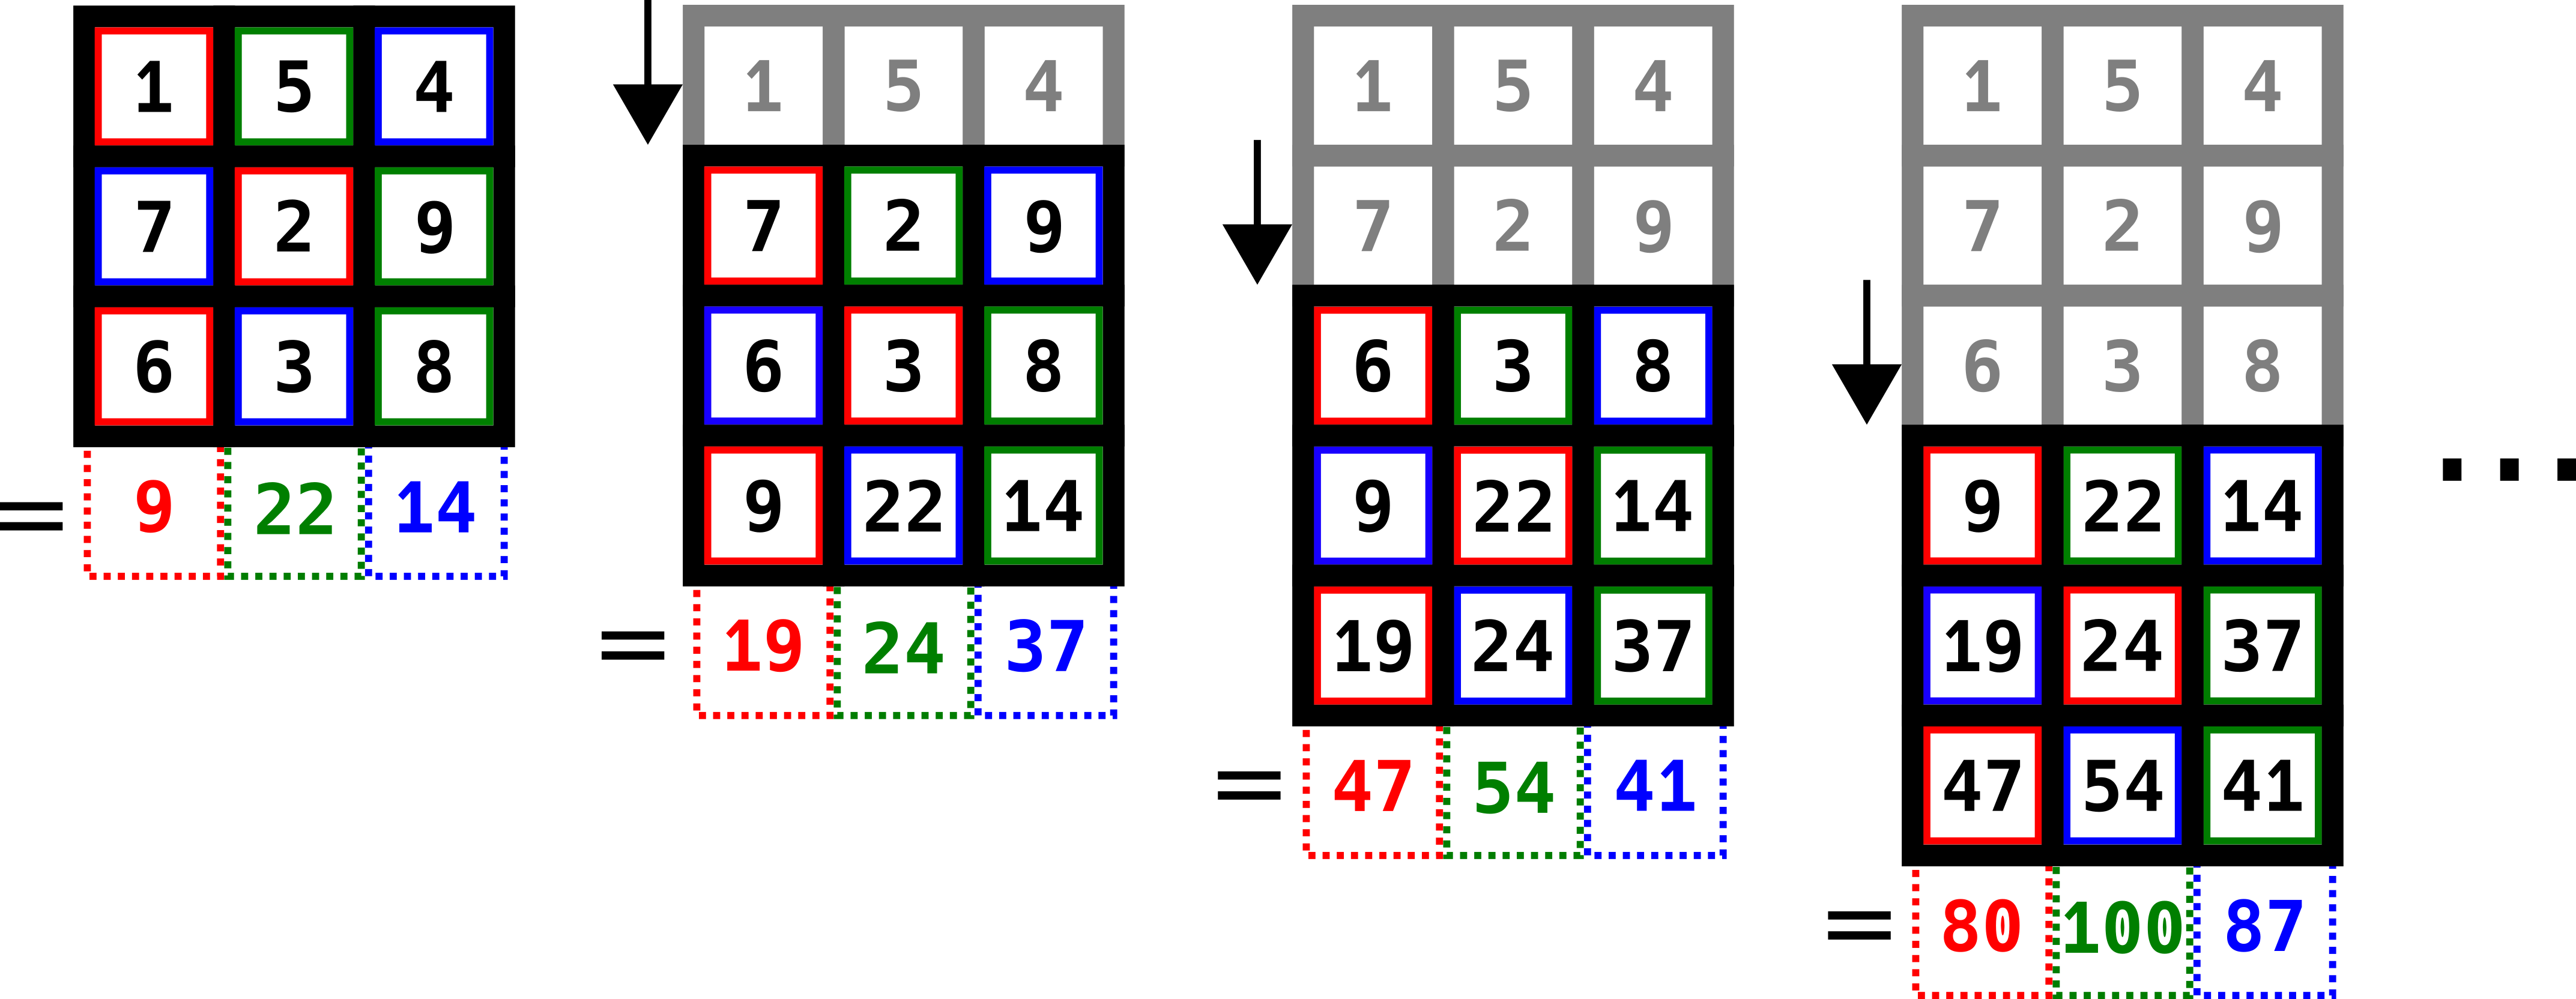
\includegraphics[scale=0.4]{kummirub/exemplo.png}
\end{center}

Liana e Hipóleto devem desenvolver uma calculadora que calcule os resultados após o $k$-ésimo turno. Você ficou responsável pelo código, e eles pelo protótipo do dispositivo, que será incluso na próxima versão do passatempo: \textit{Kummirub: 2D++!}. 

Está na hora de colocar suas habilidades de maratonista em prática! Esta primeira versão do software deverá apresentar os resultados módulo $10^9 + 7$.


\subsection*{Entrada}
A primeira linha contém o número de jogadores $N$ ($2 \leq N \leq 10$).

As próximas $N$ linhas correspondem ao tabuleiro. Cada linha contém $N$ números $C_{x, y}$ ($1 \leq C_{x, y} \leq N^2$, $0 \leq x, y < N$), o número na casa de posição ($x, y$).

A linha seguinte contém o número do turno $T$ ($1 \leq T \leq 10^8$).

Por fim, as $N$ linhas seguintes são referentes às casas escolhidas pelos jogadores. Cada linha contém $N$ números $i_{x, y}$ ($1 \leq i \leq N$), o número do jogador que escolheu a posição ($x, y$).


\subsection*{Saída}
Imprima uma linha com $N$ números $r_i$: o resultado do jogador $i$ após $T$ turnos, em módulo $10^9 + 7$.

Não coloque um espaço após o último resultado, apenas uma nova linha (`\textbackslash n').


%----- Exemplo 1 -----%
%\newpage
\begin{table}[!h]
\centering
\begin{tabular}{|l|l|}
\hline
\begin{minipage}[t]{3in}
\textbf{Exemplo de entrada}
\begin{verbatim}
3
1 5 4
7 2 9
4 3 8
4
1 2 3
3 1 2
1 3 2
\end{verbatim}
\vspace{1mm}
\end{minipage}
&
\begin{minipage}[t]{3in}
\textbf{Exemplo de saída}
\begin{verbatim}
74 96 83
\end{verbatim}
\vspace{1mm}
\end{minipage} \\
\hline
\end{tabular}
\end{table}

%----- Exemplo 2 -----%
\begin{table}[!h]
\centering
\begin{tabular}{|l|l|}
\hline
\begin{minipage}[t]{3in}
\textbf{Exemplo de entrada}
\begin{verbatim}
2
1 2
3 4
10000
2 1
1 2
\end{verbatim}
\vspace{1mm}
\end{minipage}
&
\begin{minipage}[t]{3in}
\textbf{Exemplo de saída}
\begin{verbatim}
492026538 492026538
\end{verbatim}
\vspace{1mm}
\end{minipage} \\
\hline
\end{tabular}
\end{table}


%\newpage
%\section*{L:} %tle=1
%\vspace{-0.52cm}
%\noindent \begin{verbatim}Arquivo: .[c|cpp|py]\end{verbatim}
%\input{/.tex}

\newpage
\section*{T: Tigrinho} %tle=1
\vspace{-0.52cm}
\noindent \begin{verbatim}Arquivo: tigrinho.[c|cpp|py]\end{verbatim}
Ricardinho e seu avô Gepeto estão passeando em um domingo à noite pelo circo até que se deparam com um jogo muito interessante, 
o Jogo do Tigrinho, que consiste em a partir de dois textos escritos por diferentes pessoas, determinar se um terceiro texto foi escrito ou não por uma daquelas pessoas.
De fato suas regras são bem simples:
\begin{itemize}
    \item O participante irá ler os dois primeiros textos, um de cada autor.
    \item Em seguida lê o terceiro texto, desta vez com autor desconhecido.
    \item Por fim, infere quem o escreveu sendo \textbf{1} para o primeiro, \textbf{2} para o segundo autor e \textbf{0} caso não foi escrito por nenhum deles.
    \item Os textos não precisam ter algum significado real, são apenas palavras ou sequências de letras espaçadas.
    \item Cada palavra que aparece nos textos se trata de um evento independente.
\end{itemize}

Seu papel é ajudar o Gepeto, um craque da probabilide (visto que determinada palavra tem diferentes probabilidades de 
aparição para cada autor, baseado nas evidencias fornecidas), a desvendar de quem é o texto escrito.

\subsection*{Entrada}

A primeira linha contém um número $a$ $(10 \leq a \leq 10^6)$, indicando o tamanho do texto do primeiro autor. 
Na próxima linha uma sequência de $a$ palavras com tamanho $l$ $(1 \leq l \leq 15)$ são apresentadas, correspondentes ao texto 1.

A terceira linha contém um número $b$ $(10 \leq b \leq 10^6)$, indicando o tamanho do texto do segundo autor.
Na próxima linha uma sequência de $b$ palavras com tamanho $l$ $(1 \leq l \leq 15)$ são apresentadas, correspondentes ao texto 2.

A quinta linha contém um número $n$, que indica o tamanho do texto com autor desconhecido.
E na próxima linha, $n$ palavras correspondente a este texto são apresentadas.

\subsection*{Saída}
A saída deve ser, de acordo com as probabilidades:
\begin{itemize}
    \item $1$ caso a maior probabilidade seja do primeiro autor.
    \item $2$ caso a maior probabilidade seja do segundo autor.
    \item $0$ caso a probabilidade seja 0 para ambos.
\end{itemize}
%----- Exemplo 1 -----%
\newpage
\begin{table}[!h]
\centering
\begin{tabular}{|p{4in}|p{2in}|}
\hline
\begin{minipage}[t]{3in}
\raggedright
\textbf{Exemplo de entrada} \\
\begin{verbatim}
20
um dos personagens da disney que aparece 
no filme do shrek e o pinoquio junto de 
outras famosas princesas ficticias
20
voce sabe quem foi gepeto ele e um 
personagem ficticio italiano entalhador de 
madeira idoso e pobre criador do pinoquio
7
o pinoquio foi criado pelo italiano gepeto
\end{verbatim}
\vspace{1mm}
\end{minipage}
&
\begin{minipage}[t]{3in}
\raggedright
\textbf{Exemplo de saída} \\
\begin{verbatim}
2
\end{verbatim}
\vspace{1mm}
\end{minipage}
\\ \hline
\end{tabular}
\end{table}

\begin{table}[!h]
\centering
\begin{tabular}{|p{4in}|p{2in}|}
\hline
\begin{minipage}[t]{3in}
\raggedright
\textbf{Exemplo de entrada} \\
\begin{verbatim}
86
no futebol os jogadores correm pelo campo
driblando adversarios enquanto passam a 
bola de pe em pe o objetivo principal e 
marcar um gol acertando a bola na rede 
alem da trave a preparacao fisica e mental 
e essencial para garantir bom desempenho 
o jogo e rapido exigindo precisao e 
trabalho em equipe a grama do campo e o 
palco onde a acao acontece e a vitoria e 
o sonho de todos os envolvidos cada 
segundo conta e a tecnica de controle 
da bola e crucial
81
na natacao os atletas deslizam pela agua 
avancando rapidamente pela raia a tecnica 
precisa aliada a forca e a resistencia e 
o que garante o sucesso assim como no 
futebol a preparação fisica e mental e 
indispensavel cada bracada na piscina deve 
ser calculada para maximizar a velocidade 
o tempo e um fator determinante e o 
objetivo e sempre cruzar a linha de chegada 
primeiro o ambiente de competicao como no 
campo de futebol exige foco e concentracao 
totais  dos nadadores
11
a preparacao fisica e mental e crucial 
para vencer no futebol
\end{verbatim}
\vspace{1mm}
\end{minipage}
&
\begin{minipage}[t]{3in}
\raggedright
\textbf{Exemplo de saída} \\
\begin{verbatim}
1
\end{verbatim}
\vspace{1mm}
\end{minipage}
\\ \hline
\end{tabular}
\end{table}
\newpage



\end{document}
